\documentclass[a4paper, 12pt, UTF8]{ctexart}
\usepackage{matnoble-doc-cn}
\begin{document}
\title{第二届八一杯网络大学生数学竞赛} \author{{\Large --- 代数题目若干}\\ \bf
  \href{https://matnoble.me/about/}{MatNoble}} \date{}

\maketitle
\tableofcontents

\begin{figure*}[b]
    \centering
    
\includegraphics[width = .25\textwidth]{images/logo.png}
\end{figure*}

% \clearpage

% \begin{table}[ht]
%     \normalsize
%     \centering
%     \caption{\em 命题汇总}
%     \vskip 0.1in
%     \label{table}
%     \begin{tabular}{c|l}
%       \hline
%       \hline
%       \rule{0pt}{3ex}
%       组别 & 题目编号 
%                                   \rule[-1.2ex]{0pt}{0pt} \\\hline
%       非数 & 26, 27, 53, 78   \\ 
%       数 A (高) & 12   \\
%       数 A (低) & 6, 7   \\      
%       数 B (高) & 3, 4, 5   \\
%       数 B (低) & 5   \\  
%       \hline
%       \hline 
%     \end{tabular}
% \end{table}

\clearpage

\section{线性无关的应用}

\begin{exa}
    某班级有 $n$ 位同学,共参加了 $m$ 个社团.每个社团中,该班学生的数目都是奇数;任意两个社团中,共同学生的数目是偶数.试证明: $m \leq n$. 
\end{exa}
{\color{GoogleRed}
  \begin{proof}
      令 $\bm{v}_{i} \in \mathbb{F}_{2}^{n}(i = 1, \cdots, m)$ 表示
      第 $i$ 个社团的成员信息, $\bm{v}_{i}$ 的第 $j$ 个分量
      为 $1$ 表示: 编号为 $j$ 的同学在 $i$ 社团, 反之为 $0$. 如此,
      $\bm{v}_{i}\cdot\bm{v}_{i}$ 表示第 $i$ 个社团中的人数, 由题意可
      知, 人数为偶数, 所以, 在 $\mathbb{F}_{2}$ 中,
      $\bm{v}_{i}\cdot\bm{v}_{i}=1$; 类似的,
      $\bm{v}_{i}\cdot\bm{v}_{j}(i \neq j)$ 表示同时在 $i$ 社团与 $j$
      社团的人数, 由题意可知, 人数为奇数, 所以, 在 $\mathbb{F}_{2}$ 中,
      $\bm{v}_{i}\cdot\bm{v}_{j}=0(i\neq j)$

      下面证明 $\{ \bm{v}_{1}, \cdots ,\bm{v}_{m}\}$ 是线性无关的. 假设
      存在 $c_{1}, \cdots, c_{m} \in \mathbb{F}_{2}$ 满足
      \[
          c_{1}\bm{v}_{1} + \cdots + c_{m}\bm{v}_{m} = 0.
      \]
      将 $\bm{v}_{i}(i=1,\cdots,m)$ 分别与上式作内积, 得到 $c_{i}=0(i=1,\cdots,m)$, 即 $m$ 个 $n$ 维向量线性无关, 进而得到 $m \leq n$.
      
\end{proof}
}

{\color{GoogleGreen} 非数 26}

\clearpage
\begin{exa}
    某班级有 $n$ 位同学,共参加了 $m$ 个社团.任意两个社团中,共同学生的
    数目恰 好都是 $k$ 个 $(k>0)$. 试证明: $m \leq n$.
\end{exa} {\color{GoogleRed} \begin{proof}
    令 $\bm{v}_{i}(i = 1, \cdots, m)$ 表示
      第 $i$ 个社团的成员信息, $\bm{v}_{i}$ 的第 $j$ 个向量
      为 $1$ 表示: 编号为 $j$ 的同学在 $i$ 社团, 反之为 $0$. 由题意知, $\bm{v}_{i}\cdot \bm{v}_{j} = k(i\neq j)$.

      我们知道向量 $\{\bm{v}_{1}, \cdots, \bm{v}_{m} \}$ 线性无关, 则 $m \leq n$ 成立. 反之, 则成立不全为零的 $c_{i}(i=1,\cdots,m)$ 满足
      \[
          c_{1}\bm{v}_{1} + \cdots + c_{m}\bm{v}_{m} = \bm{0}.
      \]
      对上式作如下内积,
      \[
          \begin{aligned}
            0 &= (c_{1}\bm{v}_{1} + \cdots + c_{m}\bm{v}_{m}) \cdot (c_{1}\bm{v}_{1} + \cdots + c_{m}\bm{v}_{m}) \\[3pt]
            &= \sum_{i=1}^{m}c_{i}^{2}\bm{v}_{i}\cdot\bm{v}_{i} + 2\sum_{i<j}c_{i}c_{j}\bm{v}_{i}\cdot\bm{v}_{j} \\[3pt]
            &= \sum_{i=1}^{m}c_{i}^{2}|\bm{v}_{i}|^{2} + 2k\sum_{i<j}c_{i}c_{j} \\[3pt]
            &= \sum_{i=1}^{m}c_{i}^{2}(|\bm{v}_{i}|^{2}-k) + \sum_{i=1}^{n}\sum_{j=1}^{n}c_{i}c_{j}\\[3pt]
            &= \sum_{i=1}^{m}c_{i}^{2}(|\bm{v}_{i}|^{2}-k) + \left( \sum_{i=1}^{n} c_{i}\right)^{2}
          \end{aligned}
      \]
      因为任意两个俱乐部共享 $k$ 位同学, 所以每个社团成员数不小于 $k$, 即 $|\bm{v}_{i}|^{2}-k \geq 0$. 观察上式中, 每一项都是非负数, 所以每一项的和都是 $0$. 只有当 $|\bm{v}_{i}|^{2}-k = 0$ 时的 $c_{i}$ 可以不为 $0$, 此时, $i$ 社团中恰好有 $k$ 名成员, 由题意, 这 $k$ 名成员必须参加其他所有的社团, 如此, 社团的数量最多为 $n$.
    
\end{proof}
}

{\color{GoogleGreen} 数 B 高 3, 非数 27 .本题中不同社团应理解为社团成员组成完全不同

}

\vspace{3em}

\begin{thm}{}{}
    {\adkaiti
      线性无关的题一般都需要用到 {\color{GoogleRed}$ c_{1}\bm{v}_{1} + \cdots + c_{m}\bm{v}_{m} = \bm{0}$}. 上面两道题都有现实背景, 解题思路是: 在某数域空间里构造向量组, 然后证明线性无关或相关.

      以上题目来源于 \href{https://math.mit.edu/~lmlovasz/oddtowngood.pdf}{Oddtown/Eventown 问题和 Fisher 不等式}
      }
\end{thm}

\clearpage
\section{矩阵}

\begin{exa}
    已知 $2$ 阶方阵 $
        \boldsymbol{A} = \Biggl[
        \begin{matrix}
            5 & 2 \\ 1 & 0
        \end{matrix}\Biggr]$ 
    \begin{itemize}
        \item[(i)] 方阵 $\boldsymbol{A}$ 的幂可写为: $\boldsymbol{A}^{k} = c_{k}\boldsymbol{A} + d_{k}\boldsymbol{I}, k > 0$,试计算系数 $c_{k},d_{k}$
        \item[(ii)] 试将 $\boldsymbol{A}^{-1}$ 写成 $\boldsymbol{I}$ 和 $\boldsymbol{A}$ 的线性组合
    \end{itemize}
\end{exa}

\begin{lem}{}{}
    {\adkaiti 本题考察矩阵幂的相关知识, 意在说明矩阵是由一组数按一定顺序排列形成, 但有时可以``囫囵吞枣''地认为矩阵就是一个数. 但由于笔者决定使用本题时, ``画蛇添足''地修改了数据, 导致手算很费劲, 所以, 解析中使用原数据$
\boldsymbol{A} = \bigl[\begin{smallmatrix}
          5 & 1\\
          -2& 0
      \end{smallmatrix} \bigr]
$. 本题推荐非数学或者数学系低年级同学做一做, 增加对矩阵的理解.}
\end{lem}

{\color{GoogleRed}
  \begin{solution}
      \begin{itemize}
          \item[(i)]
          矩阵 $\boldsymbol{A}$ 的特征多项式是
          $p(\lambda) = \lambda^{2} - 3\lambda +
          2$, 由 Cayley-Hamilton 定理知:
          $\boldsymbol{A}^{2} - 3\boldsymbol{A} + 2\boldsymbol{I} = 0$ 或 $\boldsymbol{A}^{2} = 3\boldsymbol{A} -
          2\boldsymbol{I}$

          已知
          $\boldsymbol{A}^{k} = c_{k}\boldsymbol{A} +
          d_{k}\boldsymbol{I}$, 那么
          $\boldsymbol{A}^{k+1} = c_{k}\boldsymbol{A}^{2} +
          d_{k}\boldsymbol{A} = c_{k}(3\boldsymbol{A} -
          2\boldsymbol{I}) + d_{k}\boldsymbol{A} = (3c_{k} +
          d_{k})\boldsymbol{A} - 2c_{k}\boldsymbol{I}$, 于是
          \[
              \begin{cases}
                  c_{k+1} &= 3c_{k} + d_{k} \\[3pt]
                  d_{k+1} &= -2c_{k}
              \end{cases}
          \]
          写成矩阵形式
          \[
              \begin{bmatrix}
                  c_{k+1}\\d_{k+1}
              \end{bmatrix} =
              \begin{bmatrix}
                  3 & 1 \\ -2 & 0
              \end{bmatrix}
              \begin{bmatrix}
                  c_{k} \\ d_{k}
              \end{bmatrix} = \boldsymbol{A}
              \begin{bmatrix}
                  c_{k} \\ d_{k}
              \end{bmatrix}
          \]
          其中, $\boldsymbol{A}$ 可以对角化
          \[
              \boldsymbol{A} = \begin{bmatrix} 3 & 1 \\ -2 & 0
              \end{bmatrix} = \boldsymbol{S\Lambda S}^{-1} =
              \begin{bmatrix}
                  1 & -1 \\ -1 & 2
              \end{bmatrix}
              \begin{bmatrix}
                  2 & 0 \\ 0 & 1
              \end{bmatrix}
              \begin{bmatrix}
                  2 & 1 \\ 1 & 1
              \end{bmatrix}
          \]
          由 $c_{0} = 0, d_{0}=1$, 得
          \[
              \begin{aligned}
                  \begin{bmatrix}
                      c_{k} \\d_{k}
                  \end{bmatrix} &= \boldsymbol{A}^{k}
                  \begin{bmatrix}
                      c_{0} \\ d_{0}
                  \end{bmatrix} =
                  \boldsymbol{S\Lambda}^{k}\boldsymbol{S}^{-1}
                  \begin{bmatrix}
                      c_{0} \\ d_{0}
                  \end{bmatrix} \\
                  &= \begin{bmatrix} 1 & -1 \\ -1 & 2
                  \end{bmatrix}
                  \begin{bmatrix}
                      2^{k} & 0 \\ 0 & 1^{k}
                  \end{bmatrix}
                  \begin{bmatrix}
                      2 & 1 \\ 1 & 1
                  \end{bmatrix}
                  \begin{bmatrix}
                      0 \\ 1
                  \end{bmatrix}
                  =
                  \begin{bmatrix}
                      2^{k} - 1 \\ -2^{k} + 2
                  \end{bmatrix}
              \end{aligned}
          \]
          \item[(ii)] 仍然利用 $\boldsymbol{A}^{2} - 3\boldsymbol{A} + 2\boldsymbol{I} = 0$, 移项
          \[
              \boldsymbol{I} = \boldsymbol{A}\biggl[ \frac{1}{2}(-2\boldsymbol{A} + 3 \boldsymbol{I}) \biggr]
          \]
          故 $\boldsymbol{A}^{-1} = \biggl[ \frac{1}{2}(-2\boldsymbol{A} + 3 \boldsymbol{I}) \biggr]$. 另外, 将 $k=-1$ 带入 (i) 中公式也可以.
      \end{itemize}
  \end{solution}
}

{\color{GoogleGreen} 数 B 高 4, 非数 53 

}

\clearpage
\begin{exa}
    假设 $\boldsymbol{A, B}$ 和 $\boldsymbol{M}$ 是 $n\times n$ 的实矩阵,满足 $\boldsymbol{AM = MB}$,并且矩阵 $\boldsymbol{A}$ 和矩阵 $\boldsymbol{B}$ 有 相同的特征多项式. 试证明: 对于任意 $n$ 阶实矩阵 $\boldsymbol{X}$ 满足 $\det(\boldsymbol{A} − \boldsymbol{MX}) = \det(\boldsymbol{B}−\boldsymbol{XM})$
\end{exa}

{\color{GoogleRed}
  \begin{proof}
      令 $\boldsymbol{A}_{\lambda} = \boldsymbol{A} - \lambda\boldsymbol{I}$, $\boldsymbol{B}_{\lambda} = \boldsymbol{B} - \lambda\boldsymbol{I}$, 由题意知, $\det (\boldsymbol{A}_{\lambda}) = \det (\boldsymbol{B}_{\lambda})$. 又因为 $\boldsymbol{AM = MB}$, 所以 $\boldsymbol{A}_{\lambda}\boldsymbol{M} = \boldsymbol{M}\boldsymbol{B}_{\lambda}$, 当 $\lambda$ 取合适值时, $\boldsymbol{A}_{\lambda}, \boldsymbol{B}_{\lambda}$ 是可逆的. 所以, $\boldsymbol{M} = \boldsymbol{A}_{\lambda}\boldsymbol{M}\boldsymbol{B}_{\lambda}^{-1}$. 令 $\boldsymbol{X}_{t} = \boldsymbol{X} + t\boldsymbol{I}$,
      \[
          \begin{aligned}
              \det(\boldsymbol{A}_{\lambda} -
              \boldsymbol{M}\boldsymbol{X}_{t}) &= \det(\boldsymbol{A}_{\lambda} -
              \boldsymbol{A}_{\lambda}\boldsymbol{M}\boldsymbol{B}_{\lambda}^{-1}\boldsymbol{X}_{t}) \\[3pt]
              &= \det(\boldsymbol{A}_{\lambda}) \det(\boldsymbol{I} - \boldsymbol{M}\boldsymbol{B}_{\lambda}^{-1}\boldsymbol{X}_{t}) \\[3pt]
              &= \det(\boldsymbol{A}_{\lambda})\det(\boldsymbol{B}_{\lambda})^{-1}\det(\boldsymbol{X}_{t})\det(\boldsymbol{X}_{t}^{-1}\boldsymbol{B}_{\lambda} - \boldsymbol{M}) \\[3pt]
              &= \det(\boldsymbol{X}_{t})\det(\boldsymbol{X}_{t}^{-1}\boldsymbol{B}_{\lambda} - \boldsymbol{M}) \\
              & = \det(\boldsymbol{B}_{\lambda} -
              \boldsymbol{X}_{t}\boldsymbol{M})
          \end{aligned}
      \]
      上式是关于 $\lambda$ 和 $t$ 的恒等式, 取 $\lambda = t = 0$ 等式仍成立, 得证.(或者, 取 $t=0$, 上式即表明 $\boldsymbol{A} − \boldsymbol{MX}$ 和 $\boldsymbol{B} − \boldsymbol{XM}$ 有相同特征多项式, 从而行列式相等)

      还可以用分块矩阵来解此题, 步骤略.
      
  \end{proof}
}

{\color{GoogleGreen} 数 B 高 5

}

\clearpage
\begin{exa}
    设 $\boldsymbol{M} =\Bigl[
    \begin{smallmatrix}
        \bm{0} & \bm{I}_{n}\\
        -\bm{I}_{n} & \bm{0}
    \end{smallmatrix}\Bigr]
$.如果实方阵 $\boldsymbol{A}$ 满足 $\boldsymbol{M}=\boldsymbol{A}^{\mathsf{T}}\boldsymbol{MA}$, 求证 $\det \boldsymbol{A} = 1$.
\end{exa}
{\color{GoogleRed}
  \begin{proof}
      假设所有满足 $\boldsymbol{M}=\boldsymbol{A}^{\mathsf{T}}\boldsymbol{MA}$ 的方阵 $\boldsymbol{A}$ 全体组成的集合为 $S$. 显然若 $\boldsymbol{A} \in S,  \boldsymbol{B} \in S$, 那么就有 $\boldsymbol{AB}\in S$. 接下来, 依次证明
      \begin{itemize}
          \item[(1)] 若 $\boldsymbol{A} \in S$, 那么 $\boldsymbol{A}^{-1} \in S, \boldsymbol{A}^{\mathsf T} \in S$.

          $\boldsymbol{A}^{-1} \in S$ 是显然的. 注意到 $\boldsymbol{M}^{2} = -\boldsymbol{I}_{2n}$, 所以
          \[
              \begin{cases}
                 (\boldsymbol{AM})\boldsymbol{M}  = (\boldsymbol{AM})\boldsymbol{A}^{\mathsf T}\boldsymbol{MA} =  (\boldsymbol{AMA}^{\mathsf T})\boldsymbol{MA}\\
                  (\boldsymbol{AM})\boldsymbol{M} = -\boldsymbol{AI}_{2n} = \boldsymbol{MMA} 
              \end{cases} \Longrightarrow \boldsymbol{M} = \boldsymbol{AMA}^{\mathsf T}
          \]
          所以, $\boldsymbol{A}^{\mathsf T} \in S$.
          \item[(2)] 若正定矩阵 $\boldsymbol{H} \in S$, 那么 $\boldsymbol{H}$ 的平方根 $\boldsymbol{P} \in S$.

          由已知得 $\boldsymbol{M} = \boldsymbol{HMH}, \boldsymbol{H}^{-1}\boldsymbol{M} = \boldsymbol{MH}$, 从而对任何多项式 $f(x)$ 有 $f(\boldsymbol{H}^{-1})\boldsymbol{M} = \boldsymbol{M}f(\boldsymbol{H})$. 设 $\boldsymbol{H}$ 特征值为 $\{ \lambda_{1}^{2}, \dots, \lambda_{2n}^{2} \}$, 正交矩阵 $\boldsymbol{O}$ 使得 $\boldsymbol{O}^{\mathsf T}\boldsymbol{HO} = {\rm diag}\{ \lambda_{1}^{2}, \dots, \lambda_{2n}^{2} \}$, 那么 $\boldsymbol{O}^{\mathsf T}\boldsymbol{PO} = {\rm diag}\{ \lambda_{1}, \dots, \lambda_{2n} \}$. 可利用拉格朗日插值法使 $f$ 满足 $f{\lambda_{i}^{2}} = \lambda_{i}, f(1/\lambda_{i}^{2})=1/\lambda_{i}$. 这样就有 $f(\boldsymbol{H}) = \boldsymbol{P}, f(\boldsymbol{H}^{-1}) = \boldsymbol{P}^{-1}$, 从而 $\boldsymbol{P} \in \boldsymbol{S}$.
          \item[(3)] 设 $\boldsymbol{A} \in S$, $\boldsymbol{A}$ 的极分解为 $\boldsymbol{A} = \boldsymbol{HQ}$, 这里 $\boldsymbol{H}$ 正定, $\boldsymbol{Q}$ 正交, 则 $\boldsymbol{H}\in S, \boldsymbol{Q}\in S$.

          $\boldsymbol{A} \in S, \boldsymbol{A}^{\mathsf T} \in S \Rightarrow \boldsymbol{AA}^{\mathsf T} \in S \Rightarrow \sqrt{\boldsymbol{AA}^{\mathsf T}} = \boldsymbol{H} \in S \Rightarrow \boldsymbol{Q} = \boldsymbol{AH}^{-1} \in S$.
          \item[(4)] 设 $\boldsymbol{Q} \in S$, $\boldsymbol{Q}$ 正交, 则 $\det \boldsymbol{Q} = 1$.

          设 $\boldsymbol{Q} =\Bigl[
          \begin{smallmatrix}
              \boldsymbol{C} & \boldsymbol{D}\\
              \boldsymbol{E} & \boldsymbol{F}
          \end{smallmatrix}\Bigr]
          $, 则 $\boldsymbol{MQ} = \boldsymbol{QM}$, 从而 $\boldsymbol{C}=\boldsymbol{F}, \boldsymbol{D} = \boldsymbol{-E}$, 所以, $\boldsymbol{Q} =\Bigl[
          \begin{smallmatrix}
              \boldsymbol{C} & \boldsymbol{D}\\
              \boldsymbol{-D} & \boldsymbol{C}
          \end{smallmatrix}\Bigr]
          $. $\boldsymbol{Q}$ 正交说明 $\boldsymbol{C}\boldsymbol{C}^{\mathsf T} + \boldsymbol{D}\boldsymbol{D}^{\mathsf T} = \boldsymbol{I}_{n}$, $\boldsymbol{CD}^{\mathsf T} = \boldsymbol{DC}^{\mathsf T}$. 从而 $(\boldsymbol{C} + i\boldsymbol{D})(\boldsymbol{C}^{\mathsf T} - i\boldsymbol{D}^{\mathsf T}) = \boldsymbol{I}_{n}$,  则
          \[
              \begin{vmatrix}
                  \boldsymbol{C} &  \boldsymbol{D}\\ - \boldsymbol{D} & \boldsymbol{C}
              \end{vmatrix} = \lvert \boldsymbol{C} + i\boldsymbol{D} \rvert \cdot \lvert \boldsymbol{C} - i\boldsymbol{D} \rvert = 1.
          \]
          从而 $\det \boldsymbol{Q} = 1$.
          \item[(5)] 设 $\boldsymbol{H} \in S$, $\boldsymbol{H}$ 正交, 则 $\det \boldsymbol{H} = 1$.

          由 $\boldsymbol{M} = \boldsymbol{HMH}$ 可得 $(\det \boldsymbol{H})^{2}=1$, 又因为 $\boldsymbol{H}$ 正定, 所以 $\det \boldsymbol{H} = 1$
      \end{itemize}
      综合 (3), (4), (5), 就得到了问题的证明.
  \end{proof}
}

{\color{GoogleGreen} 数 A 高 12, 非数 78

}

\noindent {\adheiti 优秀解答}(来自\ 戴银\ 武汉大学)

{\centering
  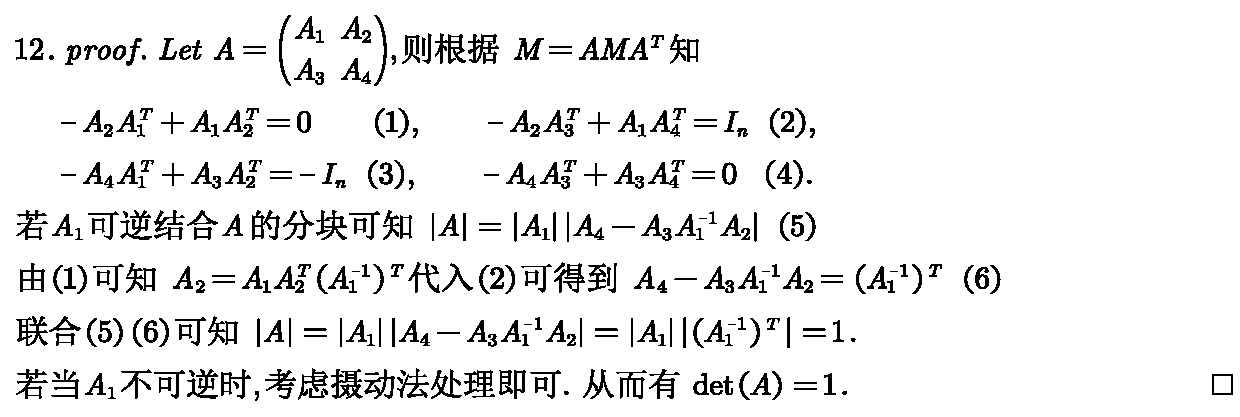
\includegraphics[width = \textwidth]{images/solution2.pdf}
}

\vspace{4em}

\begin{thm}{}{}
    {\adkaiti 矩阵是线性代数或者高等代数中的重要内容, 几乎占了半壁江山. 相应地, 矩阵的题目也是层出不穷. 作为数学竞赛, 理应相对难一些, 但考虑到全面性, 导致前两道题目稍简单, 但我认为还算有趣, 同时, 可以增加做竞赛题的信心.

      分块矩阵, 特征值, 特征向量, 特征多项式, 矩阵相似, 矩阵相抵, 矩阵相合, 矩阵对角化, 矩阵可交换, 正交矩阵, 正定矩阵, 秩 1 矩阵 ... 都是矩阵专题中重要的研究内容.

      感兴趣的同学可以买本习题集做一做(推荐亲测过的王品超的高等代数新方法)

    }
\end{thm}

\clearpage
\section{空间}

\begin{exa}
    设 $\boldsymbol{M}$ 是 $\boldsymbol{M}_{n}(\mathbb{C})$ 的一个子空
    间,如果 $\boldsymbol{M}$ 中的矩阵两两可以交换,求
    证 $\boldsymbol{M}$ 的维数最大是的 $\left[ \frac{n^{2}}{4}
    \right]+1$($\left[ \cdot \right]$ 表示高斯取整函数).
\end{exa}

{\color{GoogleRed}
  \begin{proof}
      对 $n$ 归纳, $n=1$ 结论显然成立, 设小于 $n$ 时结论也成立. 下面,
      讨论 $n$ 的情形:

      由于 $\boldsymbol{M}$ 中的矩阵两两可以交换, 所以他们可以同时上三
      角化, 所以不妨假设 $\boldsymbol{M}$ 中的每一个矩阵都是上三角矩
      阵. 对于每个 $\boldsymbol{A} \in \boldsymbol{M}$, 我们截
      取 $\boldsymbol{A}$ 左上角的 $n-1$ 阶主子阵, 把这个矩阵记
      为 $f(\boldsymbol{A})$, 同时截取 $\boldsymbol{A}$ 的右下角
      的 $n-1$ 阶主子阵, 把它记作 $g(\boldsymbol{A})$. 那么所有
      的 $f(\boldsymbol{A})$ 之间两两可以交换, 所有
      的 $g(\boldsymbol{A})$ 两两之间可以交换. 由于 $f$ 和 $g$ 都可以看
      作是 $\boldsymbol{M}$ 到 $\boldsymbol{M}_{n-1}$ 的交换子空间的线
      性映射, 所以有归纳假设,
      $\dim f \leq \left[ \frac{(n-1)^{2}}{4} \right]+1, \dim g \leq
      \left[ \frac{(n-1)^{2}}{4} \right]+1$.

      不难看出, ${\rm Ker} f$ 中的元素形如 $
      \begin{bmatrix}
          \boldsymbol{0}_{n\times n-1} & \bm{\alpha}
      \end{bmatrix}$, ${\rm Ker} g$ 中的元素形如
      $\begin{bmatrix} \bm{\beta}^{\mathsf T} \\
          \boldsymbol{0}_{n-1\times n}
      \end{bmatrix}$. 这里的 $\bm{\alpha}, \bm{\beta}$ 都是 $n$ 维列向
      量. 两者可交换意味着 $\bm{\beta}^{\mathsf T} \bm{\alpha} =
      0$, 即 ${\rm Ker} f\perp {\rm Ker} g$, 所以
      $\dim {\rm Ker} f + \dim {\rm Ker} g \geq n$, 从而
      \[
          \begin{aligned}
              \dim \boldsymbol{M} & = \dim {\rm Ker} f + \dim f =  \dim {\rm Ker} g + \dim g \\[3pt]
              &\leq \frac{\dim {\rm Ker} f + \dim {\rm Ker} g}{2} + \left[ \frac{(n-1)^{2}}{4} \right] + 1 \\[3pt]
              &\leq \frac{n}{2} + \left[ \frac{(n-1)^{2}}{4} \right] + 1 \leq \left[ \frac{(n)^{2}}{4} \right] + 1.
          \end{aligned}
      \]

      当 $n = 2m$ 是偶数时, 取形如
      \[
          \begin{bmatrix}
              \lambda \boldsymbol{I}_{m} & \boldsymbol{N}
              \\
              \boldsymbol{0} & \lambda\boldsymbol{I}_{m}
          \end{bmatrix}
      \]
      的矩阵. 当 $n = 2m+1$ 是奇数时, 取形如
      \[
          \begin{bmatrix}
              \lambda \boldsymbol{I}_{m} & \boldsymbol{N}
              \\
              \boldsymbol{0} & \lambda\boldsymbol{I}_{m+1}
          \end{bmatrix}
      \]
      的矩阵.
      
  \end{proof}
}

{\color{GoogleGreen} 数 A 低 6, 数 B 低 5

}

\noindent{\adheiti 优秀解答}(来自 Cherry 杭州师范大学)

{\centering
  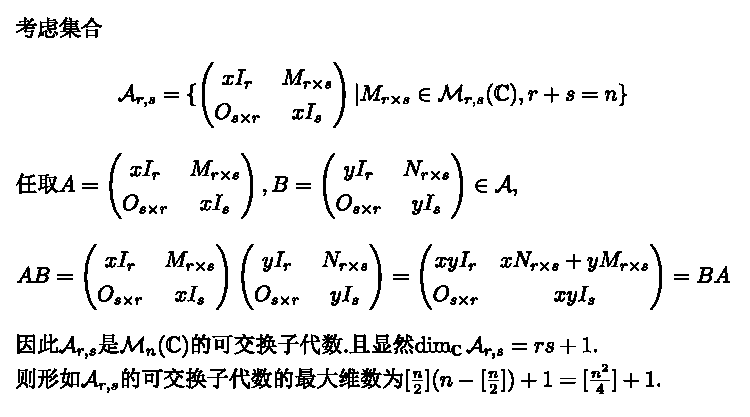
\includegraphics[width = .9\textwidth]{images/solution1.pdf}
  
}

\vspace{4em}

\begin{thm}{}{}{\adkaiti
    ``空间为体, 矩阵为用'', 空间是线性代数或高等代数中除矩阵外的又一个重要研究对象, 包括向量空间, 矩阵的四个基本空间, 子空间, 直和, 最小二乘法, 内积空间等等内容.

    类似上面的问题, 还有:
    \begin{itemize}
        \item 如果 $\boldsymbol{M}$ 中的所有矩阵的秩都不超过 $r$, 这里 $0<r<n$, 那么 $\boldsymbol{M}$ 的维数最大是多少?
        \item 如果 $\boldsymbol{M}$ 中所有矩阵都是幂零的,即对任何 $\boldsymbol{A} \in \boldsymbol{M}$, 存在一个正整数 $m$ 使得 $\boldsymbol{A}^{m}=0$, 那么 $\boldsymbol{M}$ 的维数最大是多少?
        \item 如果 $\boldsymbol{M}$ 中所有非零矩阵都是可逆矩阵,那么 $\boldsymbol{M}$ 的维数最大是多少?
    \end{itemize}

    参考链接 \href{http://pywonderland.com/subspace-of-matrices/}{矩阵空间的子空间}}
\end{thm}

\clearpage
\section{奇异值分解}
\begin{exa}
    设 $\boldsymbol{A}$ 是一个 $5 \times 4$ 阶的实矩阵,并
    且 $\boldsymbol{M}$ 有非零奇异值 $1, 2, 3, 4$,试依次计算
    \begin{enumerate}
        \item[(i)] $\det(\boldsymbol{A}^{\mathsf{T}}\boldsymbol{A})$
        \item[(ii)]
        ${\rm trace}(\boldsymbol{A}\boldsymbol{A}^{\mathsf{T}})$
        \item[(iii)]
        $\dim N(\boldsymbol{A}\boldsymbol{A}^{\mathsf{T}})$
        \item[(iv)]
        $\max_{\lVert x=1 \rVert}\lVert \boldsymbol{A}\bm{x}\rVert$
    \end{enumerate}
\end{exa}

{\color{GoogleRed}
  \begin{solution}
      设 $\boldsymbol{A}$ 的奇异值分解为
      $\boldsymbol{A = U\Sigma V}^{\mathsf
        T}$, 其中
      $\boldsymbol{UU}^{\mathsf T} = \boldsymbol{U}^{\mathsf
        T}\boldsymbol{U}=\boldsymbol{I}_{5}$,
      $\boldsymbol{VV}^{\mathsf T} = \boldsymbol{V}^{\mathsf
        T}\boldsymbol{V} = \boldsymbol{I_{4}}$,
      \[
          \Sigma = \begin{bmatrix}
              4 & 0 & 0 & 0 \\
              0 & 3 & 0 & 0 \\
              0 & 0 & 2 & 0 \\
              0 & 0 & 0 & 1 \\
              0 & 0 & 0 & 0
          \end{bmatrix}
      \]
      将奇异值分解代入计算 $\boldsymbol{A}^{\mathsf{T}}\boldsymbol{A}$
      和 $\boldsymbol{A}\boldsymbol{A}^{\mathsf{T}}$, 得到以下结果:
      \[
          \begin{aligned}
              \boldsymbol{A}^{\mathsf{T}}\boldsymbol{A} = (\boldsymbol{U\Sigma V}^{\mathsf T})^{\mathsf T}(\boldsymbol{U\Sigma V}^{\mathsf T}) = \boldsymbol{V\Sigma}^{\mathsf T} \boldsymbol{U}^{\mathsf T}\boldsymbol{U\Sigma V}^{\mathsf T} = \boldsymbol{V\Sigma}^{\mathsf T} \boldsymbol{\Sigma V}^{\mathsf T}
              \\[3pt]
              \boldsymbol{A}\boldsymbol{A}^{\mathsf{T}} = (\boldsymbol{U\Sigma V}^{\mathsf T})(\boldsymbol{U\Sigma V}^{\mathsf T})^{\mathsf T} = \boldsymbol{U\Sigma}^{\mathsf T} \boldsymbol{V}^{\mathsf T}\boldsymbol{V\Sigma U}^{\mathsf T} = \boldsymbol{U\Sigma}\boldsymbol{\Sigma}^{\mathsf T} \boldsymbol{U}^{\mathsf T}
          \end{aligned}
      \]
      其中,
      \[
          \boldsymbol{\Sigma}^{\mathsf T} \boldsymbol{\Sigma} =
          \begin{bmatrix}
              4^{2} & 0 & 0 & 0 \\
              0 & 3^{2} & 0 & 0 \\
              0 & 0 & 2^{2} & 0 \\
              0 & 0 & 0 & 1^{2}
          \end{bmatrix}, \quad
          \boldsymbol{\Sigma} \boldsymbol{\Sigma}^{\mathsf T} =
          \begin{bmatrix}
              4^{2} & 0 & 0 & 0 & 0 \\
              0 & 3^{2} & 0 & 0 & 0 \\
              0 & 0 & 2^{2} & 0 & 0 \\
              0 & 0 & 0 & 1^{2} & 0 \\
              0 & 0 & 0 & 0 & 0
          \end{bmatrix}
      \]
      \begin{itemize}
          \item[(i)]
          \[
              \begin{aligned}
                  \det(\boldsymbol{A}^{\mathsf{T}}\boldsymbol{A}) &=
                  \det( \boldsymbol{V\Sigma}^{\mathsf T}
                  \boldsymbol{\Sigma V}^{\mathsf T}) = \det(
                  \boldsymbol{V}) \det (\boldsymbol{\Sigma}^{\mathsf T}\boldsymbol{\Sigma}) \det (\boldsymbol{V}^{\mathsf T}) \\
                  &= \det(\boldsymbol{\Sigma}^{\mathsf T}
                  \boldsymbol{\Sigma}) = 4^{2} \cdot 3^{2} \cdot 2^{2}
                  \cdot 1^{2} = 576.
              \end{aligned}
          \]
          \item[(ii)] \[
              \begin{aligned}
                  {\rm
                    trace}(\boldsymbol{A}\boldsymbol{A}^{\mathsf{T}})
                  &= {\rm
                    trace}(\boldsymbol{U\Sigma}\boldsymbol{\Sigma}^{\mathsf
                    T} \boldsymbol{U}^{\mathsf T}) = {\rm
                    trace}(\boldsymbol{\Sigma}\boldsymbol{\Sigma}^{\mathsf
                    T} \boldsymbol{U}^{\mathsf T}\boldsymbol{U}) \\
                  &= {\rm trace}(\boldsymbol{\Sigma}
                  \boldsymbol{\Sigma}^{\mathsf T}) = 4^{2} + 3^{2} +
                  2^{2} + 1^{2} + 0 = 30.
              \end{aligned}
          \]
          \item[(iii)] 利用秩 -- 零化度定理, 可知
          ${\rm rank}(\boldsymbol{A}\boldsymbol{A}^{\mathsf T}) + \dim
          N(\boldsymbol{A}\boldsymbol{A}^{\mathsf{T}}) =
          5$. 因为 $\boldsymbol{U}$ 是实正交矩阵, 因此可逆, 即知
          \[
              {\rm rank}(\boldsymbol{A}\boldsymbol{A}^{\mathsf T}) =
              {\rm
                rank}(\boldsymbol{U\Sigma}\boldsymbol{\Sigma}^{\mathsf
                T} \boldsymbol{U}^{\mathsf T}) = {\rm
                rank}(\boldsymbol{\Sigma} \boldsymbol{\Sigma}^{\mathsf
                T}) = 4.
          \]
          所以,
          $\dim N(\boldsymbol{A}\boldsymbol{A}^{\mathsf T}) = 5-4=1$.
          \item[(iv)] 利用奇异值分解写出
          \[
              \begin{aligned}
                  \lVert \boldsymbol{A}\bm{x} \rVert^{2} &= (\boldsymbol{A}\bm{x})^{\mathsf T}(\boldsymbol{A}\bm{x}) = \bm{x}^{\mathsf T}\boldsymbol{A}^{\mathsf T}\boldsymbol{A} \bm{x} \\
                  &= \bm{x}^{\mathsf T} \boldsymbol{V\Sigma}^{\mathsf
                    T} \boldsymbol{\Sigma V}^{\mathsf T} \bm{x}
                  =\bm{z}^{\mathsf T} \boldsymbol{\Sigma}^{\mathsf T}
                  \boldsymbol{\Sigma} \bm{z}
              \end{aligned}
          \]
          上面令 $\bm{z}=\boldsymbol{V}^{\mathsf
            T}\bm{x}$, 就有
          $\lVert \bm{z} \rVert^{2} = \bm{z}^{\mathsf T}\bm{z} =
          \bm{x}^{\mathsf T}\boldsymbol{V}\boldsymbol{V}^{\mathsf
            T}\bm{x} = \bm{x}^{\mathsf T}\bm{x} = 1$, 因此原问题等价于
          \[
              \max_{\lVert \bm{z} \rVert=1} \sqrt{\bm{z}^{\mathsf T}
                \boldsymbol{\Sigma}^{\mathsf T} \boldsymbol{\Sigma}
                \bm{z}}
          \]
          令 $\bm{z} = [z_{1}, z_{2}, z_{3}, z_{4}]^{\mathsf T}$, 且 $z_{1}^{2} + z_{2}^{2} +z_{3}^{2}+z_{4}^{2}=1$, 可得
          \[
              \bm{z}^{\mathsf T}
                \boldsymbol{\Sigma}^{\mathsf T} \boldsymbol{\Sigma}
                \bm{z} = 4^{2}z_{1}^{2} + 3^{2}z_{2}^{2} +  2^{2}z_{3}^{2} +  1^{2}z_{4}^{2} \leq 4^{2}(z_{1}^{2} + z_{2}^{2} +z_{3}^{2}+z_{4}^{2}) = 4^{2}
            \]
            当且仅当 $\bm{z} = [1,0,0,0]^{\mathsf T}$. 所以, $\max_{\lVert x=1 \rVert}\lVert \boldsymbol{A}\bm{x}\rVert = 4$.
          
      \end{itemize}
  \end{solution}
}
{\color{GoogleGreen} 数 A 低 7

}

\vspace{4em}
\begin{thm}{}{}{\adkaiti
    奇异值分解(SVD) 是最重要的矩阵分解之一, 虽然很少出现在线性代数或者高等代数课本上, 但是奇异值分解可以解释很多线代中的其他知识, 并且应用广泛. 因此决定出一个有关奇异值分解的题目. 不太困难, 希望引起各位考友的注意.
}
\end{thm}

\vspace{4em}

最后, 若发现以上解析有错误, 请告诉我 \href{mailto:hustmatnoble@gmail.com}{hustmatnoble@gmail.com}


\end{document}
